% Research question 2 is not reviewed!
\vspace{3 mm}
\section{Proposed work}\vspace{3 mm}

As stated above, the low level drivers are provided by many third party hardware vendors so if we develop a common unit testing tool then it will benefit both Linux community and the hardware vendors by helping to harness the low level drivers and increasing the overall quality of LLDs. Hence we propose to develop one such tool which can exercise various interfaces provided by LLD with the purpose of identifying issues at unit level.  This tool will exercise the different units/interfaces of LLD with varying input combinations and make sure the LLD interfaces behave as defined by Linux SCSI community and as expected by the SML. \\

The low level driver interacts with SML in two ways.  The LLD invokes certain functions of SML and in addition it provides set of interfaces it exposes to SML through a registration process.  The picture shown below depicts the high level interactions between the LLD and SML. \\

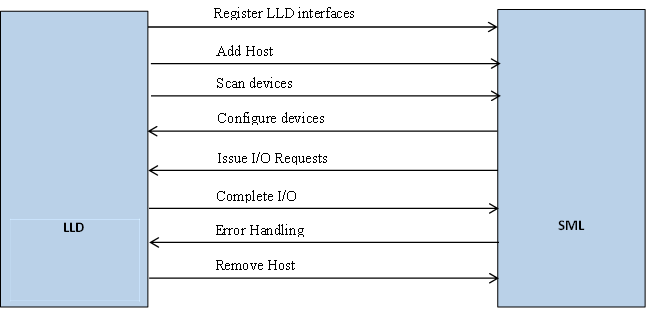
\includegraphics[scale=1]
{fig5}

We propose to introduce a new kernel module named LLD Tester (LLDT) which will be layered between LLD and SML and trap all the communication between LLD and SML. The LLDT module will then interact with SML.  By doing so, the LLDT will get control of the interfaces of LLD and can introduce new test cases or test data and execute LLD in unit test mode. 

The LLD module will also contain either CUnit/CuTest ported to kernel level and will utilize the interfaces of the Unit Test tool for test case management, test suit creation and test status update.  Since there is no way to ASSERT in kernel module the test status needs to be logged into the system logger files.

In addition to the LLD tester kernel module a user level helper application will also be developed. It will provide the context for the kernel module to run the test cases, help in configuring the test cases to run and collect test execution status.  

For introducing the LLDT, the LLD needs to be modified to a small extent, there will be a function mapper file provided by LLDT and the LLD needs to be compiled with the function mapper so that the LLD’s SML interaction can be directed to LLDT. 

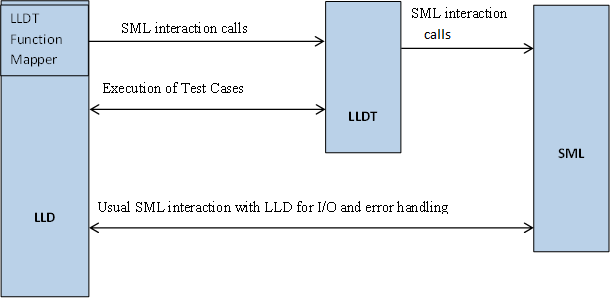
\includegraphics[scale=1]
{fig6}

The picture below shows the components of LLDT. \\

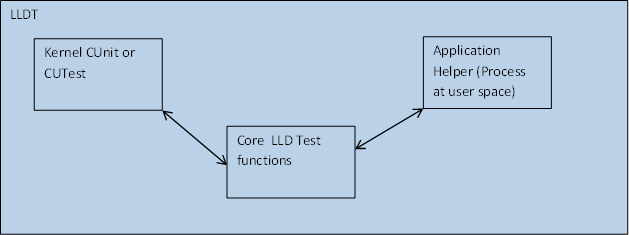
\includegraphics[scale=1]
{fig7}